%
% $RCSfile: extended_motivation.tex,v $
%
% Copyright (C) 2002-2008. Christian Heller.
%
% Permission is granted to copy, distribute and/or modify this document
% under the terms of the GNU Free Documentation License, Version 1.1 or
% any later version published by the Free Software Foundation; with no
% Invariant Sections, with no Front-Cover Texts and with no Back-Cover
% Texts. A copy of the license is included in the section entitled
% "GNU Free Documentation License".
%
% http://www.cybop.net
% - Cybernetics Oriented Programming -
%
% http://www.resmedicinae.org
% - Information in Medicine -
%
% Version: $Revision: 1.1 $ $Date: 2008-08-19 20:41:06 $ $Author: christian $
% Authors: Christian Heller <christian.heller@tuxtax.de>
%

\chapter{Extended Motivation}
\label{extended_motivation_heading}

\begin{flushright}
    \textsl{
        Those who don't have Courage to dream,\\
        will not have Power to fight.
    }\\
    \textsc{African Saying}
\end{flushright}

The previous chapters of part \ref{basics_heading} of this document investigated
state-of-the-art concepts for the development, physical- and logical architecture
of software, and some of their good and bad sides. The \emph{Suitability} of these
concepts for solving a problem, of course, heavily depends upon the intended area
of usage. This chapter introduces a new idea to software system design that is
as simple as it is helpful. It suggests to:

\begin{center}
    \textbf{Inspect solutions of various other disciplines of science,\\
    phenomenons of nature,\\
    and apply them to software engineering\\
    \ldots\ in order to find out if existing weaknesses can be eliminated.}
\end{center}

Taken as \emph{Extended Motivation} for this work, the idea leads to a new
perspective, from which traditional concepts appear in a very different light.
Former \emph{Strengths} (like the bundling of attributes and methods in an OOP
class) may suddenly be considered a \emph{Weakness}. Additionally, completely
\emph{New Conceptual Solutions} (like the unification of system communication
patterns) become possible. The merger of both, traditional and new concepts
results in the \emph{Cybernetics Oriented Programming} (CYBOP), as defined in
chapter \ref{introduction_heading}.

A description of the intended \emph{Approach} for applying
\emph{inter-disciplinary} concepts to software system design finalises this
chapter. Three topics that crystallise out here are \emph{Statics and Dynamics},
\emph{Knowledge Schema} and \emph{State and Logic}. They are explained together
with their parallels to science or nature in part \ref{contribution_heading}
following afterwards, which represents the actual \emph{Core} of this document.

%
% $RCSfile: idea.tex,v $
%
% Copyright (C) 2002-2008. Christian Heller.
%
% Permission is granted to copy, distribute and/or modify this document
% under the terms of the GNU Free Documentation License, Version 1.1 or
% any later version published by the Free Software Foundation; with no
% Invariant Sections, with no Front-Cover Texts and with no Back-Cover
% Texts. A copy of the license is included in the section entitled
% "GNU Free Documentation License".
%
% http://www.cybop.net
% - Cybernetics Oriented Programming -
%
% http://www.resmedicinae.org
% - Information in Medicine -
%
% Version: $Revision: 1.1 $ $Date: 2008-08-19 20:41:07 $ $Author: christian $
% Authors: Christian Heller <christian.heller@tuxtax.de>
%

\section{Idea}
\label{idea_heading}

Researchers quite often follow the approach of first looking into what nature
offers and then trying to engineer a similar solution. All kinds of tools and
machines were created this way, even (and most obviously, with respect to the
human body and mind) robots and computers. Some scientists take the principles
of human awareness as physical model to explain the \emph{Universe} \cite{ripota}.
Some business people and consultants see analogies between processes in the
human brain and \emph{Organisational Structures of a Company} \cite{schoenhofer}.
Researchers in human sciences systematise \emph{International Public Law} by
sharing it into the three parts \emph{Society}, \emph{Cooperation} and
\emph{Conflicts} which are chosen in analogy to biology, that is \emph{Anatomy},
\emph{Physiology} and \emph{Pathology} of international relations \cite{bierzanek}.

Considering all that, one question is at hand: \textit{Why not apply a similar
approach to software engineering?} If computers are built after the model of
the human being (information input, memorising, processing and output), why not
structure the software that actually \emph{runs} those computers after similar
models? It seems logical and clear, yet the reality looks different. This work
wants to change that, and thereby help to improve application programming.

In search for new concepts to structure software, other sciences are called in.
The idea to marry systems sciences (notably general systems theory and cybernetics)
for analysis with creative problem solving techniques of designers for synthesis
is not new. Swift \cite{designmatrix} for example tried to apply both in form of
\emph{Cyberpatterns} to complex systems problems, using a pattern language. Yet
while Swift had turned his attention to what he calls \textit{the extreme front
end}, this work goes one step further. It applies the principles of nature
(results of many different sciences) not only to the \emph{User Interface}
(frontend) of an application, but to whole software system architectures.

\begin{figure}[ht]
    \begin{center}
        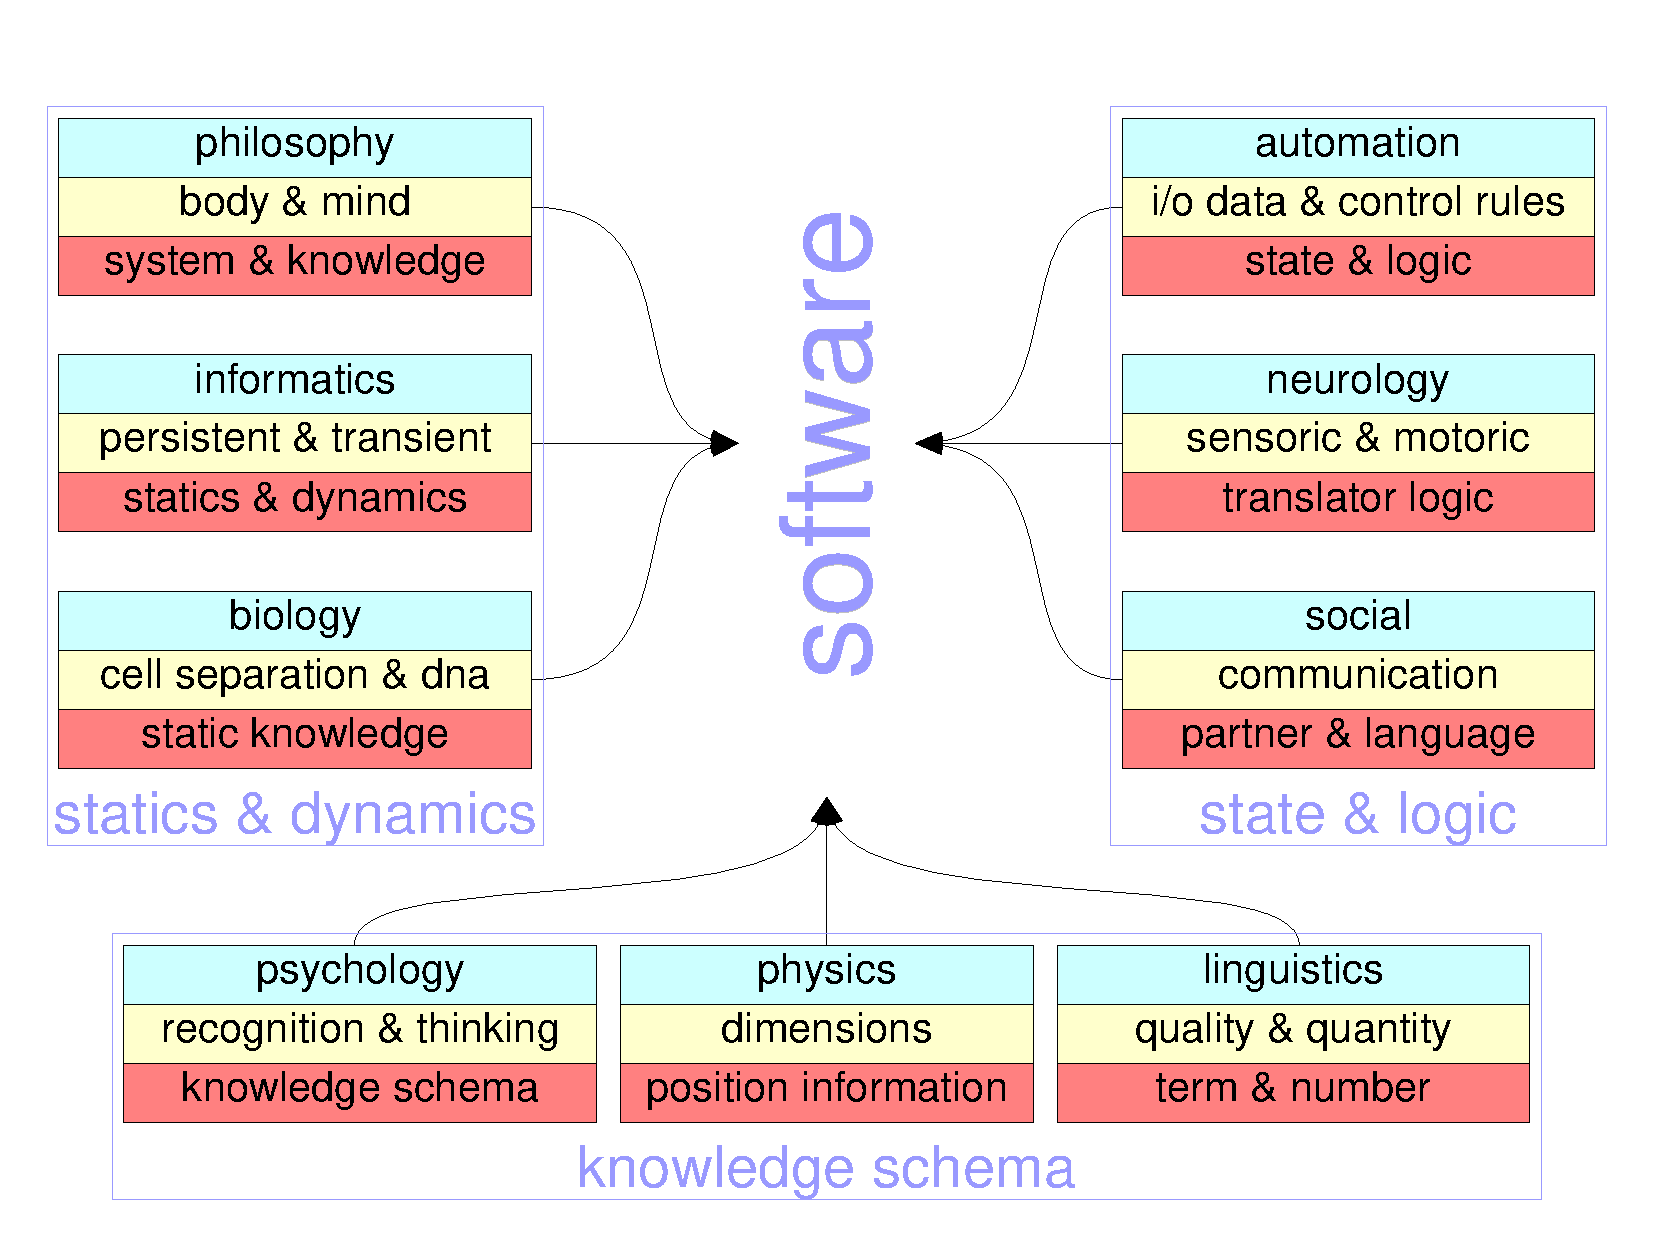
\includegraphics[scale=0.3,angle=-90]{graphic/mindmap.pdf}
        \caption{Mindmap of Sciences whose Principles influenced CYBOP}
        \label{mindmap_figure}
    \end{center}
\end{figure}

Figure \ref{mindmap_figure} shows some of the sciences whose principles were
considered in this work. The name of a field of science is shown on top of each
box. Made observations are mentioned below, in the middle. The resulting design
recommendations for software can be found at the bottom of each box. The
recommendations are grouped into those that justify a separation of
\emph{Statics and Dynamics} (left-hand side), a new kind of
\emph{Knowledge Schema} (lower part of the figure) and a distinction between
\emph{State and Logic} models (right-hand side).

It has to be mentioned though, that only some of the principles underlying a
specific field of science were considered in the figure and in more detail
later in this work. The figure does by no means claim to be complete. The shown
observations are only those that seemed promising in the context of software
design. The existence of persistent and transient data, for example, is only
one of many aspects of the science of informatics. Similarly is the existence
of sensoric and motoric nerve system just one aspect of the field of neurology.
And so on. Further details on the mentioned sciences and observations are not
given here, since later chapters will elaborate on them.

%
% $RCSfile: recapitulation.tex,v $
%
% Copyright (C) 2002-2008. Christian Heller.
%
% Permission is granted to copy, distribute and/or modify this document
% under the terms of the GNU Free Documentation License, Version 1.1 or
% any later version published by the Free Software Foundation; with no
% Invariant Sections, with no Front-Cover Texts and with no Back-Cover
% Texts. A copy of the license is included in the section entitled
% "GNU Free Documentation License".
%
% http://www.cybop.net
% - Cybernetics Oriented Programming -
%
% http://www.resmedicinae.org
% - Information in Medicine -
%
% Version: $Revision: 1.2 $ $Date: 2008-09-07 15:36:07 $ $Author: christian $
% Authors: Christian Heller <christian.heller@tuxtax.de>
%

\section{Recapitulation}
\label{recapitulation_heading}

The concepts that were found by considering other scientific disciplines, reveal
a number of state-of-the-art software design solutions that do not comply with
their original in nature, for example the:

\begin{enumerate}
    \item Mix of static application knowledge and instructions for dynamic
        system control (chapter \ref{statics_and_dynamics_heading})
    \item False combination of information ignoring hierarchical structure and
        mixing in meta information (chapter \ref{knowledge_schema_heading})
    \item Bundling of state- and logic knowledge (chapter
        \ref{state_and_logic_heading})
\end{enumerate}

\newpage

These discrepancies are the major reason for the issues mentioned in section
\ref{motivation_heading}. They become clearer only later in this work (part
\ref{contribution_heading}), where more background knowledge will be provided.
Almost all problems they cause have their root in \emph{Dependencies}. As a
system grows, the inter-dependencies between its single parts grow with. Why
does this happen? Simply because a clear architecture is missing. Even if
developers really try to follow a such -- on some point in the software's
lifetime, compromises have to be made due to unforeseen requirements and
dependencies:

\begin{itemize}
    \item[-] \emph{Meta Techniques} are used to provide basic functionality
    \item[-] \emph{Static Managers} accessible by any other parts in the system
        are introduced
    \item[-] \emph{Multiple Interfaces} are implemented to realise new
        properties (\emph{Mix-In})
    \item[-] \emph{Redundant Code} needs to be written to avoid too many
        unwanted inter-dependencies
    \item[-] \emph{Varying Mechanisms} are applied to plugin new software layers
\end{itemize}

It seems that today's software models rarely abstract the real world correctly.
This is \emph{not} general criticism on software development as it exists today,
\emph{nor} is it criticism on the abilities of application developers who use
current concepts and languages. It is just the neutral, unbiased realisation
that there are a few concepts in use which cause unclear, unnecessary, wrong
dependencies within software systems. The application of principles of other
scientific disciplines might have the potential to solve that.

It was early that, in the style of \emph{Bionics}, parallels between computing
machines and the human brain were seen, yet unfortunately do both not function
in exactly the same manner. Concepts like \emph{Artificial Neural Networks} (ANN)
%(section \ref{artificial_neural_networks_heading})
that try to imitate the
physical structure of the human brain exist, but are today's computers with
deterministic behaviour not built like that; they often have a
\emph{von Neumann Architecture} \cite{philippow}. This forces human programmers
to \emph{adapt} their thinking to the machine concepts.

Traditional programming languages and design solutions try to ease application
development by bridging the gap between concepts of human thinking and those of
the machine. Software developers are given tools to design programs in a more
abstract way, independently from the source code which gets generated later.
But as long as the underlying concepts of abstraction are insufficient, design
problems are to be expected. The kind and quality of abstractions is so
important, because it influences -- and \emph{is} influenced by -- all aspects
of software development (part \ref{basics_heading}) dealing with
\emph{Knowledge}:

\begin{itemize}
    \item[-] the \emph{Software Engineering Process} specifies static knowledge
        models (abstractions resulting from process phases), to be later
        dynamically processed in a computer system
    \item[-] the \emph{Physical Architecture} requires the translation of
        knowledge models (communication) between systems
    \item[-] the \emph{Logical Architecture} provides the means to represent
        knowledge models (by languages and various techniques) within a system
\end{itemize}

They all, consciously or not, are trials to apply human patterns. The structure
of knowledge models, for example, is based on concepts of \emph{Human Thinking},
the logical \emph{Mind} -- as opposed to the above-mentioned neural networks
that want to imitate the functioning of the physical \emph{Brain}. Because of
the central importance of knowledge, one aim of this work is to investigate new
techniques for its abstraction, to thereby revise state-of-the-art software
development. However, probably not all traditional concepts will be thrown
away. Basic things like control structures (looping, branching etc.)
abstracting logic knowledge in form of algorithms are still of importance but
appear in a different form (as will be shown in chapter
\ref{cybernetics_oriented_language_heading}). It therefore seems to be more
suitable to say that the new concepts will complement (and not revise
completely) existing development techniques, as was planned at the beginning of
this work (figure \ref{method_figure}).

%
% $RCSfile: approach.tex,v $
%
% Copyright (c) 2005-2006. Christian Heller. All rights reserved.
%
% Permission is granted to copy, distribute and/or modify this document
% under the terms of the GNU Free Documentation License, Version 1.1 or
% any later version published by the Free Software Foundation; with no
% Invariant Sections, with no Front-Cover Texts and with no Back-Cover
% Texts. A copy of the license is included in the section entitled
% "GNU Free Documentation License".
%
% http://www.cybop.net
% - Cybernetics Oriented Programming -
%
% http://www.resmedicinae.org
% - Information in Medicine -
%
% Version: $Revision: 1.1 $ $Date: 2006-01-03 08:21:45 $ $Author: christian $
% Authors: Christian Heller <christian.heller@tuxtax.de>
%

\section{Approach}
\label{approach_heading}

On its way to solving the issues mentioned in sections
\ref{introduction_heading} and \ref{architectural_troubles_heading}, the
work followed the \emph{Cybernetics Oriented Programming} (CYBOP) approach
\cite{heller2004}. The idea behind is as simple as it is helpful; it suggests
to:

\begin{center}
    Inspect solutions of various disciplines\\
    of science, phenomenons of nature,\\
    and apply them to software engineering.
\end{center}

Figure \ref{mindmap_figure} shows some sciences whose principles were
considered in this work. The name of a field of science is shown on top of each
box. Made observations are mentioned below, in the middle. The resulting design
recommendations for software can be found at the bottom of each box. The
recommendations are grouped into those that justify a distinction between
\emph{Statics and Dynamics}, a new kind of \emph{Knowledge Schema} and a
separation of \emph{State- and Logic} models.

\begin{figure}[ht]
    \begin{center}
        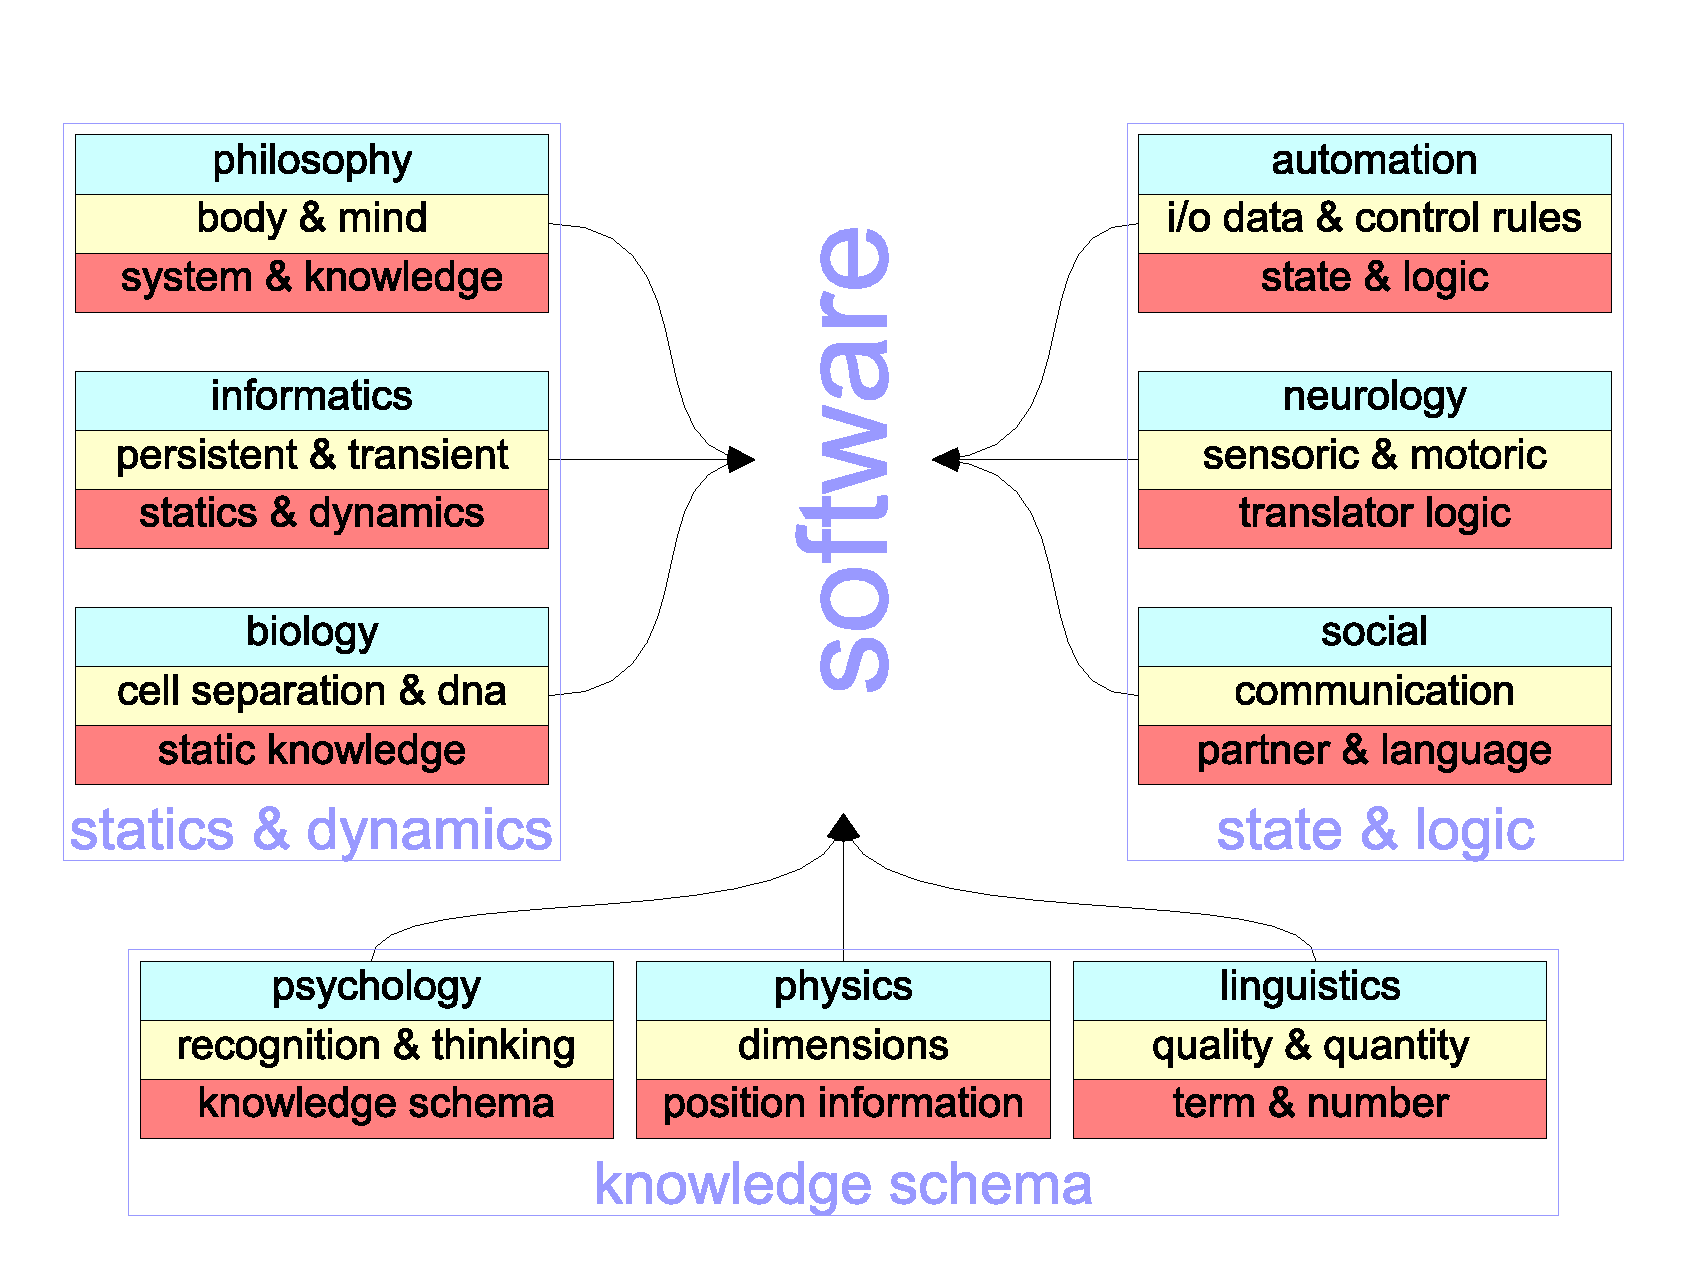
\includegraphics[scale=0.2]{vector/mindmap.eps}
        \caption{Mindmap of Influential Sciences}
        \label{mindmap_figure}
    \end{center}
\end{figure}

\begin{figure}[ht]
    \begin{center}
        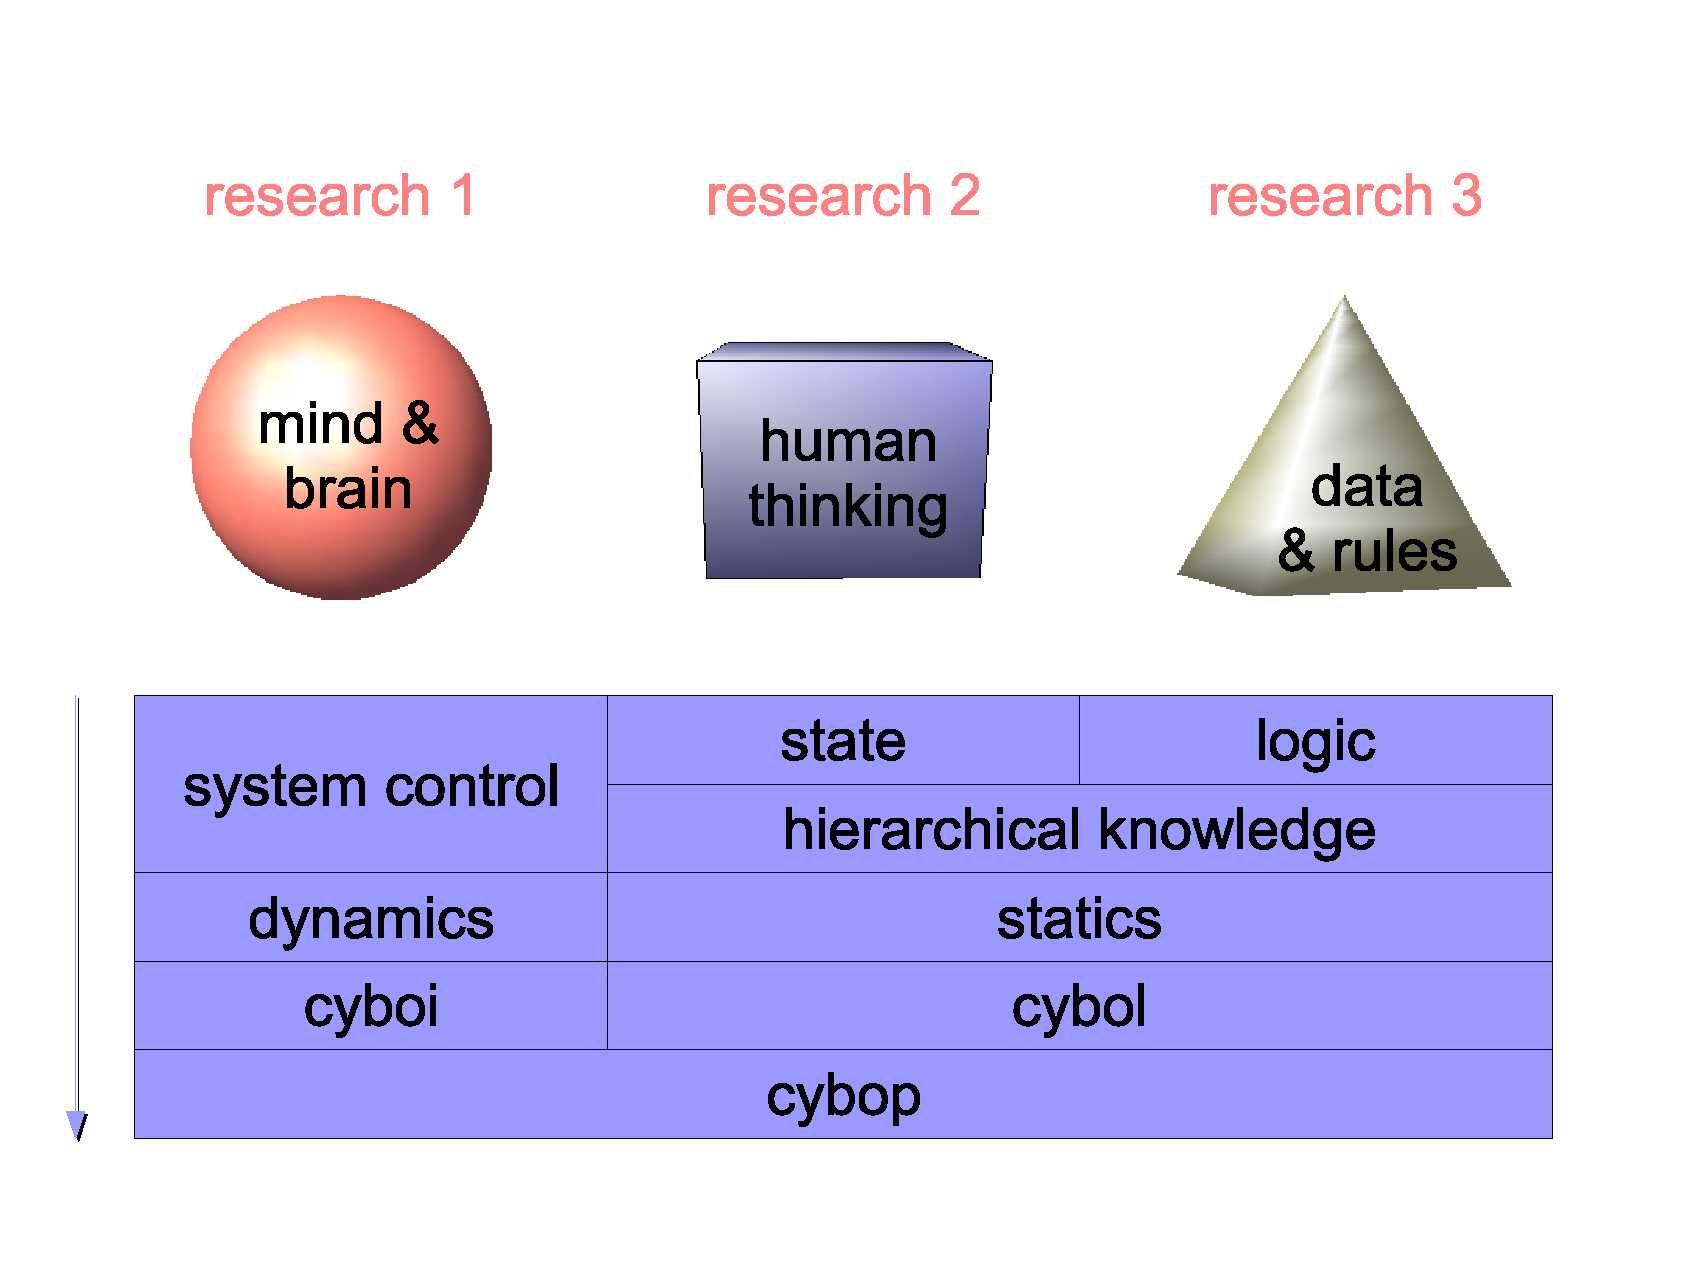
\includegraphics[scale=0.2]{vector/approach.eps}
        \caption{Overall CYBOP Approach}
        \label{approach_figure}
    \end{center}
\end{figure}

A first observation, when looking at human beings from a philosophical
perspective, is the separation of \emph{Mind} and \emph{Brain} (Body).
Accordingly, CYBOP treats computers as \emph{Systems} owning and processing
\emph{Knowledge}. This is not unlike the idea of \emph{Agent} systems owning a
\emph{Knowledge Base} \cite{parks, kuehnel}. All abstract knowledge that humans
make up belongs to their mind. The brain is merely a physical carrier of
knowledge. Similarly, there are actually two kinds of software: one
representing \emph{passive} knowledge and the other \emph{actively} controlling
a system's hardware.

Secondly, attention is payed to the concepts of \emph{Human Thinking}
\cite{heller2004}, as investigated by psychology. Through their application,
knowledge becomes \emph{hierarchical}. Moreover, this work tries to embed
knowledge models in an environment of \emph{Dimensions}, as known from physics.
Every model keeps a number of \emph{Meta Information} about its parts.
\emph{Positions} in space or time are one such example.

Thirdly, \emph{State-} gets distinguished from \emph{Logic} knowledge. It is
known from neurological research that the human brain has special communication
regions that, simply spoken, do nothing else than translating data, i.e. an
input- into an output \emph{State}, according to rules of \emph{Logic}. Systems
theory uses similar abstractions. When talking about states, this work means a
composed \emph{Set} of states.

In CYBOP (figure \ref{approach_figure}), all knowledge (states and logic),
belongs to a system's \emph{Statics}, and is described by CYBOL language
templates (section \ref{practical_proof_heading}). The processing of knowledge
at runtime, to control a system, is \emph{Dynamics} and happens in the CYBOI
interpreter.

